\documentclass{article}
\pagestyle{empty}
\usepackage{tikz,amsmath}
\usetikzlibrary{arrows,positioning}
\usepackage[margin=1in]{geometry}
\setlength{\parindent}{0in}
\newcommand{\blk}[1]{\rule{.5cm}{0cm}$#1$\rule{.5cm}{0cm}}

\begin{document}
Name\hrulefill Student Number\hrulefill \\
CSCI321, Fall 2017, Pop Quiz \#6


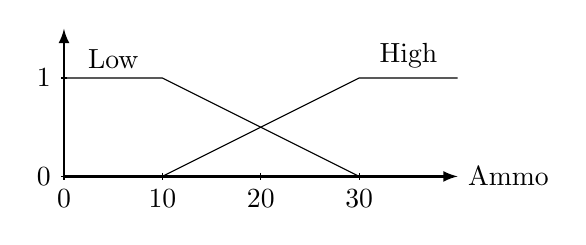
\begin{tikzpicture}[scale=1.25]
  \draw[thick,->,>=latex] (0,0) -- (4,0) node[anchor=west] {Ammo};
  \draw[thick,->,>=latex] (0,0) -- (0,1.5);
  \foreach \x in {0,10,20,30}
    \draw (\x mm,1pt) -- (\x mm,-1pt) node[anchor=north] {$\x$};
  \foreach \y in {0,1}
    \draw (1pt,\y cm) -- (-1pt, \y cm) node[anchor=east] {$\y$};
    \draw (0,1) -- node[anchor=south]{Low} (1,1) -- (3,0);
    \draw (1,0) -- (3,1) -- node[anchor=south]{High} (4,1);
\end{tikzpicture}
\hfill
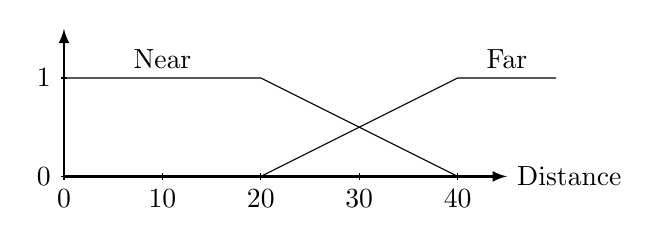
\begin{tikzpicture}[scale=1.25]
  \draw[thick,->,>=latex] (0,0) -- (4.5,0) node[anchor=west] {Distance};
  \draw[thick,->,>=latex] (0,0) -- (0,1.5);
  \foreach \x in {0,10,20,30,40}
    \draw (\x mm,1pt) -- (\x mm,-1pt) node[anchor=north] {$\x$};
  \foreach \y in {0,1}
    \draw (1pt,\y cm) -- (-1pt, \y cm) node[anchor=east] {$\y$};
    \draw (0,1) -- node[anchor=south]{Near} (2,1) -- (4,0);
    \draw (2,0) -- (4,1) -- node[anchor=south]{Far} (5,1);
\end{tikzpicture}


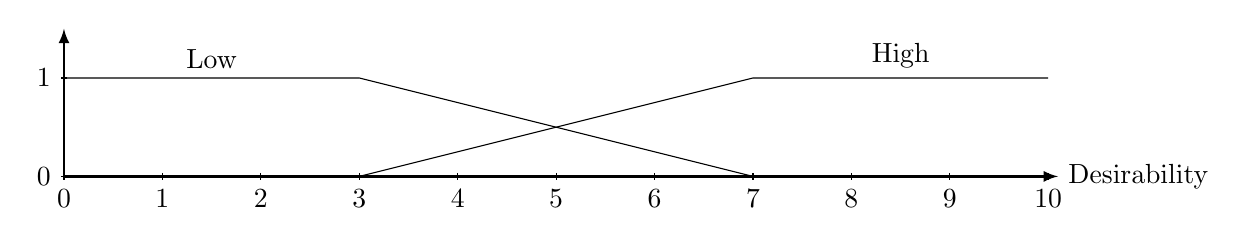
\begin{tikzpicture}[scale=1.25]
  \draw[thick,->,>=latex] (0,0) -- (10.1,0) node[anchor=west] {Desirability};
  \draw[thick,->,>=latex] (0,0) -- (0,1.5);
  \foreach \x in {0,1,2,3,4,5,6,7,8,9,10}
    \draw (\x cm,1pt) -- (\x cm,-1pt) node[anchor=north] {$\x$};
  \foreach \y in {0,1}
    \draw (1pt,\y cm) -- (-1pt, \y cm) node[anchor=east] {$\y$};
    \draw (0,1) -- node[anchor=south]{Low} (3,1) -- (7,0);
    \draw (3,0) -- (7,1) -- node[anchor=south]{High} (10,1);
\end{tikzpicture}


\newcommand{\myrule}[3]{If ammo is {\bf #1} and target is {\bf #2}
  then desirability
  is {\bf #3}. \vfill}
Given the FLVs for a weapon shown above, calculate the fuzzy
desirability for the weapon from each of the following rules,
given that ammo=25 and distance=25. 
\begin{enumerate}
\item \myrule{low}{near}{low}
\item \myrule{low}{far}{high}
\item \myrule{high}{near}{high}
\item \myrule{high}{far}{low}
\end{enumerate}

What is the final fuzzy value of desirability by combining all rules?

\vfill

\end{document}
